\section{Аналитическая часть}

\subsection{Цель и задачи}
\underline{Цель данной работы} - разработать межсетевой экран, осуществляющий контроль проходящего через него сетевого трафика, в виде загружаемого модуля.

Необходимо предоставить пользователю возможность задания правил фильтрации пакетов и изменения видимости модуля в системе.

Для достижения поставленной цели необходимо решить следующие задачи:
\begin{enumerate}
	\item изучить основные принципы работы сети и межсетевых экранов;
	
	\item ознакомиться со способом перехвата пакетов сети;
	
	\item проанализировать особенность misc драйвера и основные принципы работы с ним;
	
	\item реализовать межсетевой экран. \newline
\end{enumerate}

\subsection{Общие принципы работы сети}
\textbf{Компьютерная сеть} -- совокупность компьютеров и других устройств, соединённых линиями связи и обменивающихся информацией между собой в соответствии с определёнными правилами -- \textbf{протоколами}. \cite{net}

Информация преобразуется в пакеты и передаётся от одного компьютера к другому, и для этого используются протоколы. Каждый пакет проходит несколько стадий, которые определены в модели OSI (наглядно представлена в виде таблицы \ref{osi_table}).

\begin{table}[h]
	\begin{center}
		\caption{Модель OSI}
		\label{osi_table}
		\begin{tabular}{| p{1cm} | p{7cm} |}
			\hline
			\textbf{№} 	& \textbf{Название} \\
			\hline
			7 				& Прикладной уровень\\ 
			\hline
			6 				& Уровень представления  \\ 
			\hline
			5 		& Сеансовый уровень \\ 
			\hline
			4 		& Транспортный уровень \\ 
			\hline
			3 		& Сетевой уровень \\ 
			\hline
			2 		& Канальный уровень \\ 
			\hline
			1 		& Физический уровень \\ 
			\hline
		\end{tabular}
	\end{center}
\end{table} 

\newpage

Из пакета можно получить различную информацию, такую как:
\begin{itemize}
	\item IP source – IP-адрес источника;
	
	\item IP destination – IP-адрес назначения;
	
	\item source port - порт источника;
	
	\item destination port - порт назначения (для известных сервисов порты зарезервированы и известны заранее);
	
	\item TCP/UDP - протоколы транспортного уровня;
	
	\item другое. \\
\end{itemize}

Для каждого приложения ведутся две системные очереди: очередь данных, поступающих к приложению из сети, и очередь данных, отправляемых этим приложением в сеть. Такие очереди называются \textbf{портами}, причём входная и выходная очереди одного приложения рассматриваются как один порт. Для идентификации портов им присваивают номера. \newline

\subsection{Межсетевой экран}
\textbf{Межсетевой экран} -- это программное средство, предназначенное для фильтрации входящего и исходящего трафика, в соответствии с некоторыми заранее заданными критериями, правилами, тем самым, осуществляя защиту компьютера от сетевых угроз. 

В общих чертах его работа изображена на Рисунке \ref{fig1:image}.

\begin{figure}[ph!]
	\centering
	\begin{center}
		{\includegraphics[scale=0.5]{img/firewall.jpg}}
		\caption{Принцип работы межсетевого экрана}
		\label{fig1:image}
	\end{center}
\end{figure}

Межсетевой экран в основном работает на пакетном уровне (уровни 3 и 4 модели OSI, которая представлена в таблице \ref{osi_table}). \cite{fw}

Пакеты могут анализироваться в соответствии со следующими критериями: 
\begin{itemize}
	\item формальная корректность пакета;
	\item направление (входящий или исходящий);
	\item тип протокола;
	\item порт (источника, назначения);
	\item и т.д. \\
\end{itemize}

Для того, чтобы отфильтровать пакеты по тому или иному признаку, необходимо задать соответствующие правила, которые создаются пользователем. Когда межсетевой экран перехватывает пакет, он просматривает все его поля и сравнивает их с правилами из таблицы, причём в том порядке, как они были заданы. Если совпадение было найдено, то пакет дальше никуда не передаётся. \newline

\subsection{Загружаемый модуль ядра}
Для того, чтобы добавить новый функционал в ядро Linux, нужно либо перекомпилировать его (что небезопасно), либо воспользоваться загружаемым модулем ядра. \cite{os}

После загрузки модуля он становится частью операционной системы и ему доступны все структуры и функции ядра. Когда функциональность, предоставляемая модулем, больше не требуется, то он может быть выгружен.

В Linux все модули обычно хранятся в каталоге /lib/modules и имеют расширение .ko. Модули загружаются и выгружаются с помощью специальных команд, приведённых в Листинге \ref{lst:module}.

\begin{lstlisting}[caption = {Команды для загрузки и выгрузки загружаемого модуля ядра}, label=lst:module]
// загрузить модуль в ядро
insmod <имя модуля.ko>
		
// выгрузить модуль из ядра
rmmod <имя модуля>
\end{lstlisting}

Загружаемый модуль ядра должен иметь определённую структуру. Обязательной частью любого загружаемого модуля являются.
\begin{itemize}
	\item \textbf{Функция загрузки (инициализации) модуля.} В заголовке используется макрос \_\_init\_\_. Её задачей является подготовка модуля для дальнейшего функционирования как части ядра ОС.
	
	\item \textbf{Функция выгрузки модуля.} В заголовке используется макрос \_\_exit\_\_. Его задачей является освобождение ресурсов, занимаемых модулем в конце его работы. 
	
	\item \textbf{Макросы module\_init(init\_func), module\_exit(exit\_func)} нужны для формирования кода, который будет выполняться при загрузке/выгрузке модуля (в частности внутри этого кода содержится вызов функций \_\_init\_\_ и \_\_exit\_\_, переданных в макросы).
	
	\item \textbf{Макрос MODULE\_LICENSE(char* license)} сообщает, под какой лицензией находится модуль. Обычно указывается "GPL".
\end{itemize}
Приведённые первые две функции являются \textbf{точками входа}. Также в модуле может быть указано следующее.
\begin{itemize}
	\item \textbf{MODULE\_AUTHOR("Name"), MODULE\_DESCRIPTION("LAB")} -- макросы, определяющие информацию о модуле (имя автора, краткое описание).
	
	\item \textbf{Дополнительные точки входа.} Это можно сделать, например, с помощью структуры file\_operations, где можно указать функции модуля в качестве точек входа в него при различных действиях с файлом. \newline
\end{itemize}

\subsection{Изменение видимости модуля}
Для того, чтобы посмотреть все загруженные модули можно воспользоваться командой \textbf{lsmod}, которая читает /proc/modules и отображает информацию о файле (название, размер, сколько раз и какой модуль использует его) в отформатированном списке. \cite{lsmod}

Модуль описывается в системе с помощью структуры \textbf{struct module} (Листинг \ref{lst:struct_module}).
\begin{lstlisting}[caption = {struct module}, label=lst:struct_module]
	struct module
	{
		enum module_state state;
		struct list_head list; /* Member of list of modules */
		char name[MODULE_NAME_LEN]; /* Unique handle for this module */
		...
	};
\end{lstlisting}

В этой структуре содержится поле list -- элемент связного списка модулей. При загрузке ядро добавляет модуль в список. При выгрузке, наоборот, исключает. 

Скрытие модуля подразумевает в себе задачу удаления соответствующего элемента из этого списка. А восстановление видимости, наоборот, добавление.

Для взаимодействия со списком модулей необходимо использовать структуру \textbf{struct list\_head} и функции \textbf{list\_add}, \textbf{list\_del}. Перед тем, как удалить модуль, следует сохранить указатель, чтобы можно было восстановить его видимость. \cite{hide} \newline

\subsection{Управление внешними устройствами}
Одна из самых сложных задач системы -- управление внешними устройствами. Их достаточно много (мыши, клавиатуры, сканеры, принтеры и т.д.), все разных типов и выполняют разные задачи.  

Структура \textbf{struct file\_operations} (Листинг \ref{lst:file_op}) используется для определения собственных функций для работы с конкретным устройством. 
\begin{lstlisting}[caption = {struct file\_operations}, label=lst:file_op]
struct file_operations {
	struct module *owner;
	...
	ssize_t (*read) (struct file *, char __user *, size_t, loff_t *);
	ssize_t (*write) (struct file *, const char __user *, size_t, loff_t *);
	...
	int (*open) (struct inode *, struct file *);
	...
	int (*release) (struct inode *, struct file *);
	...
}
\end{lstlisting}

Файл устройства -- это специальный файл, который обеспечивает связь между файловой системой и драйверами устройств. В отличие от обычных файлов они являются только указателями на соответствующие драйверы в ядре.

Файлы устройств имеют три дополнительных атрибута, которые характеризуют устройство, соответствующее данному файлу:
\begin{enumerate}
	\item \textbf{класс устройства}:
	\begin{itemize}
		\item блок-ориентированные (блочные) (пример: жёсткий диск) передают данные блоками, взаимодействие только через буферную память;
		\item байт-ориентированные (символьные) (пример: принтер) передают данные посимвольно, как непрерывный поток байт, для взаимодействия буфер не требуется;
	\end{itemize}

	\item \textbf{старший номер} устройства, обозначающий тип устройства (посмотреть их можно в /proc/devices);
	
	\item \textbf{младший номер} устройства применяется для нумерации устройств одного типа, т. е. устройств с одинаковыми старшими номерами.
\end{enumerate}

Для того, чтобы идентифицировать устройство, используются старший и младший номера. \cite{os} \newline

\subsection{Драйвер в ОС Linux}
\textbf{Драйвер} -- особая программа, является частным случаем загружаемого модуля ядра.  Есть отличительная особенность -- множество точек входа (более 2), и все определены в соответствующей структуре. Основная задача драйвера -- управление внешними устройствами. \cite{os}

В Linux драйверы делятся на 3 типа:
\begin{enumerate}
	\item \textbf{встроенные в ядро}
	
	\item \textbf{реализованные как загружаемые модуля ядра};
	
	\item \textbf{код модулей поделён между ядром и специальной утилитой}
\end{enumerate}

Межсетевой экран -- драйвер второго типа, поскольку может быть свободно загружен и выгружен пользователем. \newline

\subsubsection{Misc Device Driver}
\textbf{Misc} (от слова "miscellaneous") \textbf{драйвером} называется простой символьный драйвер. Его используют в случаях, когда возможно использовать упрощение: не задавать самостоятельно старший номер устройства (major), поскольку он определён заранее и равен 10. Но разработчик должен задать младший номер в пределах от 1 до 255. \cite{2nd,misc}

Такой подход позволяет сэкономить оперативную память, особенно, если необходимо создать несколько символьных драйверов для нескольких простых устройств.

На misc драйверах могут быть определены операции open, read, write, close и т.д. И так же создаётся файл /dev/\{misc\_file\}.

По аналогии с символьными драйверами, которые описываются структурой struct cdev, misc драйверы описываются с помощью структуры \textbf{struct miscdevice}, поля которой приведены в Листинге \ref{lst:misc}.
\begin{lstlisting}[caption = {struct miscdevice}, label=lst:misc]
struct miscdevice {
	int minor;
	const char *name;
	struct file_operations *fops;
	umode_t i_mode;
	struct miscdevice *next, *prev;
};
\end{lstlisting}

Поле minor может принимать значение MISC\_DYNAMIC\_MINOR, означающее, что он будет назначен автоматически. \cite{3d}

Для работы с таким драйвером используются функции, представленные в Листинге \ref{lst:misc_reg}.
\begin{lstlisting}[caption = {Функции для регистрации и удаления misc драйвера}, label=lst:misc_reg]
	// регистрация драйвера
	int misc_register(struct miscdevice *misc);
	
	// удаление драйвера
	int misc_deregister(struct miscdevice *misc);
\end{lstlisting}

\subsection{netfilter}
netfilter -- это механизм фильтрации сетевых пакетов, который позволяет отслеживать их перемещение и при необходимости можно перехватить, блокировать. \cite{hook} \newline

\subsubsection{Точки перехвата}
Путь сетевого пакета в ядре изображен на Рисунке \ref{fig2:image}. \\

\begin{figure}[ph!]
	\centering
	\begin{center}
		{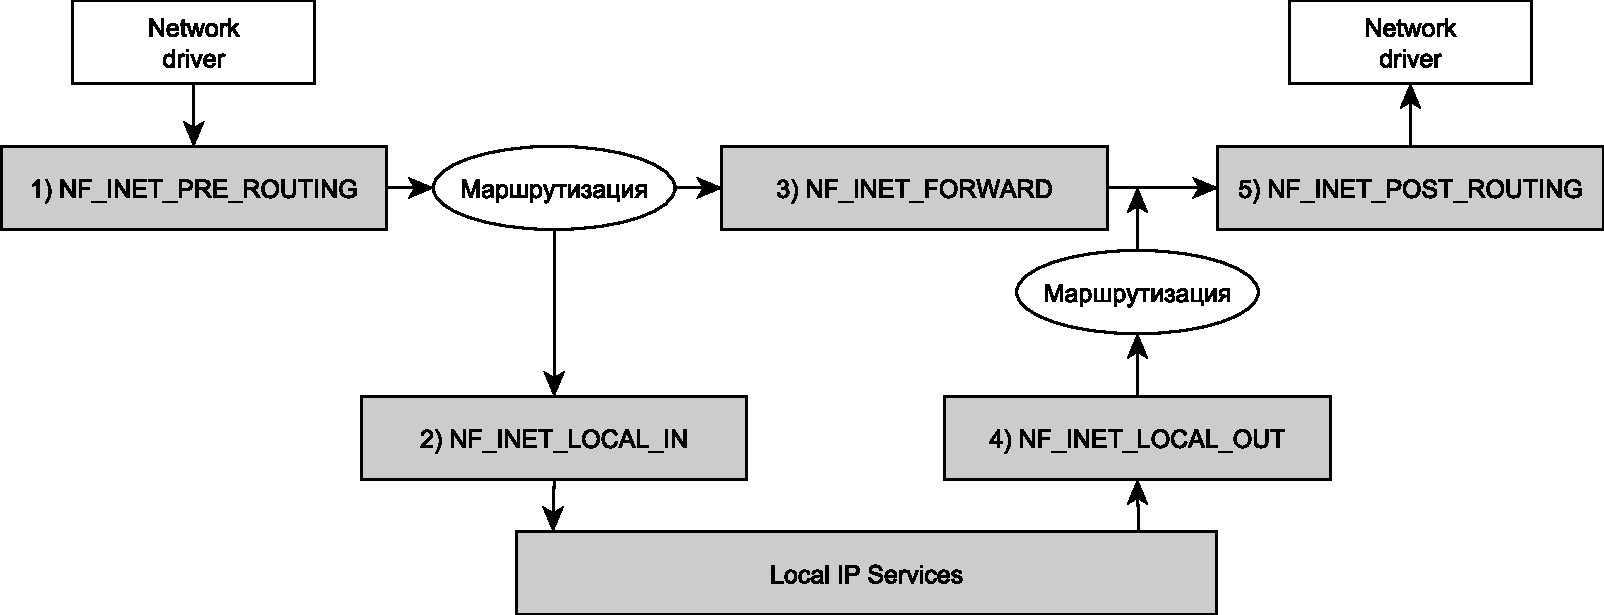
\includegraphics[scale=0.6]{img/packets.pdf}}
		\caption{Путь сетевого пакета}
		\label{fig2:image}
	\end{center}
\end{figure}

Предоставляется 5 точек, на которых могут быть определены функции перехвата, которые называются \textbf{хук-функциями}:
\begin{enumerate}
	\item NF\_INET\_PRE\_ROUTING – для всех входных пакетов;
	\item NF\_INET\_LOCAL\_IN – используется, чтобы перехватить пакеты, предназначенные для локального процесса;
	\item NF\_INET\_FORWARD – используется для пакетов, предназначенных для другого интерфейса;
	\item NF\_INET\_LOCAL\_OUT – для пакетов, которые создают локальные процессы;
	\item NF\_INET\_POST\_ROUTING – для пакетов, которые уже настроены для дальнейшего прохождения по сети к своему адресату и готовы покинуть текущий сетевой стек. \newline
\end{enumerate}

\subsubsection{Хук-функции}
Для того, чтобы использовать хук-функцию, необходимо сначала заполнить структуру \textbf{struct nf\_hook\_ops}. Структура с основными полями приведена в Листинге \ref{lst:hook}.

\begin{lstlisting}[caption = {struct nf\_hook\_ops}, label=lst:hook]
struct nf_hook_ops {
	nf_hookfn			*hook;
	...
	u_int8_t			pf;
	unsigned int		hooknum;
	int					priority;
};
\end{lstlisting}

В структуре находятся следующие поля:
\begin{itemize}
	\item \textbf{hook} -- функция, которая будет вызвана для обработки пакета, принимается решение отбросить или принять пакет;
	
	\item \textbf{pf} -- семейство протоколов;
	
	\item \textbf{hooknum} -- точка перехвата;
	
	\item \textbf{priority} -- приоритет. \\
\end{itemize}

Регистрация и удаление хуков осуществляется посредством вызова функций, которые представлены в Листинге \ref{lst:hook_reg}.

\begin{lstlisting}[caption = {Функции для регистрации и удаления хук-функций}, label=lst:hook_reg]
	// регистрация
	int nf_register_net_hook(struct net *net, const struct nf_hook_ops *ops);
	
	// удаление
	void nf_unregister_net_hook(struct net *net, const struct nf_hook_ops *ops);
\end{lstlisting}

\subsection{Выводы из аналитического раздела}
В этом разделе были сформулированы цель и необходимые для её достижения задачи, рассмотрены основные этапы, также подробно изучены принципы работы межсетевого экрана. 

Для достижения поставленной цели было принято решение использовать простой misc драйвер, поскольку он ориентирован на выполнение небольших задач и имеет упрощённую схему создания.


 